% MIT License
%
% Copyright (c) 2021 Geoffrey H. Garrett
%
% Permission is hereby granted, free of charge, to any person obtaining a copy
% of this software and associated documentation files (the "Software"), to deal
% in the Software without restriction, including without limitation the rights
% to use, copy, modify, merge, publish, distribute, sublicense, and/or sell
% copies of the Software, and to permit persons to whom the Software is
% furnished to do so, subject to the following conditions:
%
% The above copyright notice and this permission notice shall be included in all
% copies or substantial portions of the Software.
%
% THE SOFTWARE IS PROVIDED "AS IS", WITHOUT WARRANTY OF ANY KIND, EXPRESS OR
% IMPLIED, INCLUDING BUT NOT LIMITED TO THE WARRANTIES OF MERCHANTABILITY,
% FITNESS FOR A PARTICULAR PURPOSE AND NONINFRINGEMENT. IN NO EVENT SHALL THE
% AUTHORS OR COPYRIGHT HOLDERS BE LIABLE FOR ANY CLAIM, DAMAGES OR OTHER
% LIABILITY, WHETHER IN AN ACTION OF CONTRACT, TORT OR OTHERWISE, ARISING FROM,
% OUT OF OR IN CONNECTION WITH THE SOFTWARE OR THE USE OR OTHER DEALINGS IN THE
% SOFTWARE.

%%%%%%%%%%%%%%%%%%%%%%%%%%%%%%%%%%%%%%%%%%%%%%%%%%%%%%%%%%%%%%%%%%%%%%%%%%%%%%%
% ACKNOWLEDGEMENTS
%%%%%%%%%%%%%%%%%%%%%%%%%%%%%%%%%%%%%%%%%%%%%%%%%%%%%%%%%%%%%%%%%%%%%%%%%%%%%%%
% Design and implementation of this diagram was inspired and adapted from:
% https://tex.stackexchange.com/questions/104334/tikz-diagram-of-a-perceptron

%%%%%%%%%%%%%%%%%%%%%%%%%%%%%%%%%%%%%%%%%%%%%%%%%%%%%%%%%%%%%%%%%%%%%%%%%%%%%%%
% DEPENDENCIES
%%%%%%%%%%%%%%%%%%%%%%%%%%%%%%%%%%%%%%%%%%%%%%%%%%%%%%%%%%%%%%%%%%%%%%%%%%%%%%%
%\usepackage{tikz}
%\usetikzlibrary{decorations.pathreplacing}    % for TikZ braces
\usetikzlibrary{positioning}                  % for TikZ relative positioning

%%%%%%%%%%%%%%%%%%%%%%%%%%%%%%%%%%%%%%%%%%%%%%%%%%%%%%%%%%%%%%%%%%%%%%%%%%%%%%%
% USER STYLING
%%%%%%%%%%%%%%%%%%%%%%%%%%%%%%%%%%%%%%%%%%%%%%%%%%%%%%%%%%%%%%%%%%%%%%%%%%%%%%%

% TikZ node design.
\tikzset{basic/.style={draw,text width=1em,text badly centered}}
\tikzset{input/.style={basic, fill=green!25, circle}}
\tikzset{output/.style={basic, fill=blue!25, circle}}
\tikzset{weight/.style={basic,circle}}
\tikzset{hidden/.style={basic,circle}}
\tikzset{function/.style={basic,circle}}

\def\layersep{4.5em}
\def\layerseg{0.9em}
\def\transferx{9em}
\def\hiddenx{7em}
\def\hiddenxn{12em}

% Labels and symbols.
\def\activationlabel{threshold step}       % activation function label
\def\activationsymbol{$H$}                 % activation function symbol
\def\transferlabel{sum}                    % transfer function label
\def\transfersymbol{$\sum$}                   % transfer function symbol
\def\outputsymbol{$\text{OR}(x_1, x_2)$}   % output symbol
\def\inputsymbol{$x$}                      % input symbol
\def\inputvecsymbol{$\mathbf{x}$}          % input vector symbol
\def\weightslabel{weights}                 % input vector symbol
\def\biassymbol{$b$}                       % bias symbol

\def\sep{4em}
\def\L{\gls{L}}       % number of hidden layers
\def\y{\gls{y_true}}  % output vector
\def\x{\gls{ml:x}}    % input vector
\def\h{\gls{a_vec}}   % hidden output
\def\nx{\gls{np:dim}[_\gls{fn:in}]}   % hidden output
\def\ny{\gls{np:dim}[_\gls{fn:out}]}   % hidden output
\def\z{\gls{dl:z}}   % hidden output
\def\a{\gls{dl:a}}   % hidden output

%%%%%%%%%%%%%%%%%%%%%%%%%%%%%%%%%%%%%%%%%%%%%%%%%%%%%%%%%%%%%%%%%%%%%%%%%%%%%%%
% TIKZ PICTURE
%%%%%%%%%%%%%%%%%%%%%%%%%%%%%%%%%%%%%%%%%%%%%%%%%%%%%%%%%%%%%%%%%%%%%%%%%%%%%%%
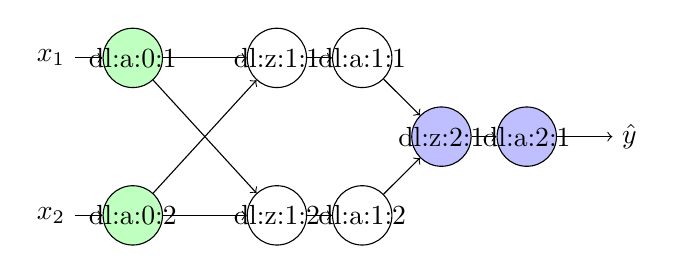
\begin{tikzpicture}

    \node[] at ({\transferx}, 0)                                                               (a1-center)   {};
    \node[left=\layersep of a1-center]                                                         (x-center)    {};

    \node[hidden, above of=a1-center, label={[xshift=-0.0em]center:\gls{dl:z:1:1}}]            (z11)         {\phantom{\gls{dl:z:1:1}}};
    \node[hidden, right=\layerseg of z11, label={[xshift=-0.0em]center:\gls{dl:a:1:1}}]        (a11)         {\phantom{\gls{dl:a:1:1}}};

    \node[hidden, below of=a1-center, label={[xshift=-0.0em]center:\gls{dl:z:1:2}}]            (z12)         {\phantom{\gls{dl:z:1:2}}};
    \node[hidden, right=\layerseg of z12, label={[xshift=-0.0em]center:\gls{dl:a:1:2}}]        (a12)         {\phantom{\gls{dl:a:1:2}}};

    \node[output, right=\layersep of a1-center, label={[xshift=-0.0em]center:\gls{dl:z:2:1}}]  (z21)         {\phantom{\gls{dl:z:2:1}}};
    \node[output, right=\layerseg of z21, label={[xshift=-0.0em]center:\gls{dl:a:2:1}}]        (a21)         {\phantom{\gls{dl:a:2:1}}};

    \node[right=2em of a21]                                                                    (out)         {$\hat{y}$};
%
    \node[input, above of=x-center, label={[xshift=-0.0em]center:\gls{dl:a:0:1}}]              (a01)         {\phantom{\gls{dl:a:0:1}}};
    \node[input, below of=x-center, label={[xshift=-0.0em]center:\gls{dl:a:0:2}}]              (a02)         {\phantom{\gls{dl:a:0:2}}};
%    \node[input, below of=x-center] (a02) {};
    \node[, left=1em of a01]          (x-1) {$x_1$};
    \node[, left=1em of a02]          (x-2) {$x_2$};

    \path[draw,->] (x-1) -- (a01);
    \path[draw,->] (x-2) -- (a02);

    \path[draw,->] (a01) -- (z12);
    \path[draw,->] (a02) -- (z12);
    \path[draw,->] (z12) -- (a12);

    \path[draw,->] (a01) -- (z11);
    \path[draw,->] (a02) -- (z11);
    \path[draw,->] (z11) -- (a11);

    \path[draw,->] (a12) -- (z21);
    \path[draw,->] (a11) -- (z21);
    \path[draw,->] (z21) -- (a21);

    \path[draw,->] (a21) -- (out);


\end{tikzpicture}
